\documentclass{article}\usepackage[]{graphicx}\usepackage[]{color}
%% maxwidth is the original width if it is less than linewidth
%% otherwise use linewidth (to make sure the graphics do not exceed the margin)
\makeatletter
\def\maxwidth{ %
  \ifdim\Gin@nat@width>\linewidth
    \linewidth
  \else
    \Gin@nat@width
  \fi
}
\makeatother

\definecolor{fgcolor}{rgb}{0.345, 0.345, 0.345}
\newcommand{\hlnum}[1]{\textcolor[rgb]{0.686,0.059,0.569}{#1}}%
\newcommand{\hlstr}[1]{\textcolor[rgb]{0.192,0.494,0.8}{#1}}%
\newcommand{\hlcom}[1]{\textcolor[rgb]{0.678,0.584,0.686}{\textit{#1}}}%
\newcommand{\hlopt}[1]{\textcolor[rgb]{0,0,0}{#1}}%
\newcommand{\hlstd}[1]{\textcolor[rgb]{0.345,0.345,0.345}{#1}}%
\newcommand{\hlkwa}[1]{\textcolor[rgb]{0.161,0.373,0.58}{\textbf{#1}}}%
\newcommand{\hlkwb}[1]{\textcolor[rgb]{0.69,0.353,0.396}{#1}}%
\newcommand{\hlkwc}[1]{\textcolor[rgb]{0.333,0.667,0.333}{#1}}%
\newcommand{\hlkwd}[1]{\textcolor[rgb]{0.737,0.353,0.396}{\textbf{#1}}}%

\usepackage{framed}
\makeatletter
\newenvironment{kframe}{%
 \def\at@end@of@kframe{}%
 \ifinner\ifhmode%
  \def\at@end@of@kframe{\end{minipage}}%
  \begin{minipage}{\columnwidth}%
 \fi\fi%
 \def\FrameCommand##1{\hskip\@totalleftmargin \hskip-\fboxsep
 \colorbox{shadecolor}{##1}\hskip-\fboxsep
     % There is no \\@totalrightmargin, so:
     \hskip-\linewidth \hskip-\@totalleftmargin \hskip\columnwidth}%
 \MakeFramed {\advance\hsize-\width
   \@totalleftmargin\z@ \linewidth\hsize
   \@setminipage}}%
 {\par\unskip\endMakeFramed%
 \at@end@of@kframe}
\makeatother

\definecolor{shadecolor}{rgb}{.97, .97, .97}
\definecolor{messagecolor}{rgb}{0, 0, 0}
\definecolor{warningcolor}{rgb}{1, 0, 1}
\definecolor{errorcolor}{rgb}{1, 0, 0}
\newenvironment{knitrout}{}{} % an empty environment to be redefined in TeX

\usepackage{alltt}

%
% Paquets basics: posar-los sempre
%
\usepackage[utf8]{inputenc}
\usepackage[T1]{fontenc}
%\usepackage[spanish, catalan]{babel}
\usepackage[english,spanish]{babel}
\usepackage{url}
%\usepackage[pdftex]{graphicx}
\usepackage{underscore}


% 
% Paquets opcionals: posar-los quan sapiguem si cale i que coi fan ...
%
\usepackage{times}
\usepackage{amsmath}
\usepackage{amssymb,amsfonts,textcomp}
\usepackage{array}
\usepackage{hhline}


% \textwidth=6.2in
% \textheight=8.5in
% %\parskip=.3cm
% \oddsidemargin=.1in
% \evensidemargin=.1in
% \headheight=-.3in



\newcommand{\R}{\textbf{R}\,}
\newcommand{\RFI}{\textbf{R}}

\newcommand{\Rfun}[1]{{\texttt{#1}}}
\newcommand{\Robj}[1]{{\texttt{#1}}}
\newcommand{\Rpac}[1]{{\textit{#1}}}   
\newcommand{\Rfunction}[1]{{\texttt{#1}}}
\newcommand{\Robject}[1]{{\texttt{#1}}}
\newcommand{\Rpackage}[1]{{\textit{#1}}}
\newcommand{\Rclass}[1]{{\textit{#1}}}
\newcommand{\bit}{\begin{itemize}}
\newcommand{\eit}{\end{itemize}}
\newcommand{\ben}{\begin{enumerate}}
\newcommand{\een}{\end{enumerate}}

\newcommand{\classdef}[1]{%
  {\em #1}
}

\begin{knitrout}
\definecolor{shadecolor}{rgb}{0.969, 0.969, 0.969}\color{fgcolor}\begin{kframe}
\begin{alltt}
\hlstd{opts_chunk}\hlopt{$}\hlkwd{set}\hlstd{(}\hlkwc{fig.path}\hlstd{=}\hlstr{'images/grafic'}\hlstd{,} \hlkwc{tidy}\hlstd{=}\hlnum{FALSE}\hlstd{,} \hlkwc{dev}\hlstd{=}\hlstr{'pdf'}\hlstd{)}
\end{alltt}
\end{kframe}
\end{knitrout}


\begin{knitrout}
\definecolor{shadecolor}{rgb}{0.969, 0.969, 0.969}\color{fgcolor}\begin{kframe}
\begin{alltt}
\hlstd{workingDir} \hlkwb{<-} \hlkwd{getwd}\hlstd{()}
\hlstd{dataDir} \hlkwb{<-} \hlkwd{file.path}\hlstd{(workingDir,} \hlstr{"dades"}\hlstd{)}
\hlstd{resultsDir} \hlkwb{<-} \hlkwd{file.path}\hlstd{(workingDir,} \hlstr{"results"}\hlstd{)}
\hlstd{codeDir} \hlkwb{<-}\hlkwd{file.path}\hlstd{(workingDir,} \hlstr{"Rcode"}\hlstd{)}
\hlkwd{setwd}\hlstd{(workingDir)}

\hlkwd{options}\hlstd{(}\hlkwc{width}\hlstd{=}\hlnum{80}\hlstd{)}
\hlkwd{options}\hlstd{(}\hlkwc{digits}\hlstd{=}\hlnum{5}\hlstd{)}

\hlstd{toPNG} \hlkwb{<-} \hlnum{FALSE}
\end{alltt}
\end{kframe}
\end{knitrout}

\title{Building and validating predictors using \R}

\author{Alex Sánchez\\
Estad\'istica i Bioinform\`atica\\
Department d'Estadística. Universitat de Barcelona}

\bibliographystyle{plain}

% \includeonly{file1, file2, ...} % Por si se quiere romper el documento en subdocumentos elaborables separadamente
\IfFileExists{upquote.sty}{\usepackage{upquote}}{}
\begin{document}




\section{Introduction}

A common task in bioinformatics is tu build and validate a predictor
to distinguish between two or more biological classes based on a
series of biological features such as genes, microRNA, metabolites (or,
more recently, a combination of some of these).

Our goal here is to illustrate the \emph{standard process} such as
described by Sanchez et alt. (\cite{Sanchez2013}) or by Serra Cayuela (\cite{SerraCayuela2015}) and summarized
in the follwing two figures.

Figure \ref{workflow} illustrates the basics blocks on which the biomarker discovery process can be arbitrarily divided. Figure \ref{validation} illustrates how to use cross-validation to build and validate a biomarker in such a way that unbiased estimates of generalization error can be obtained.

\begin{figure}
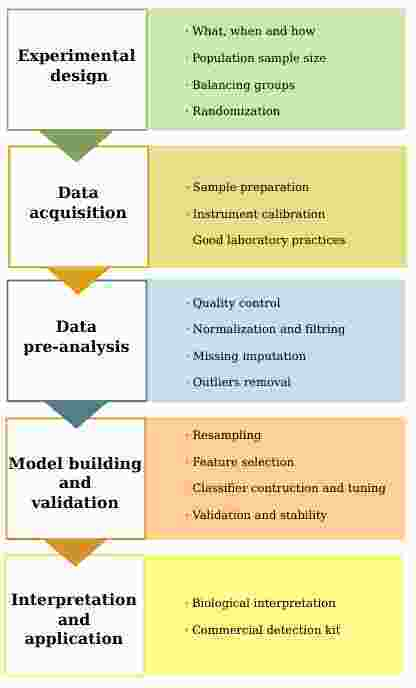
\includegraphics[width=10cm]{images/biomarkerDiscoveryWorkflow}
\label{workflow}
\end{figure}


\begin{figure}
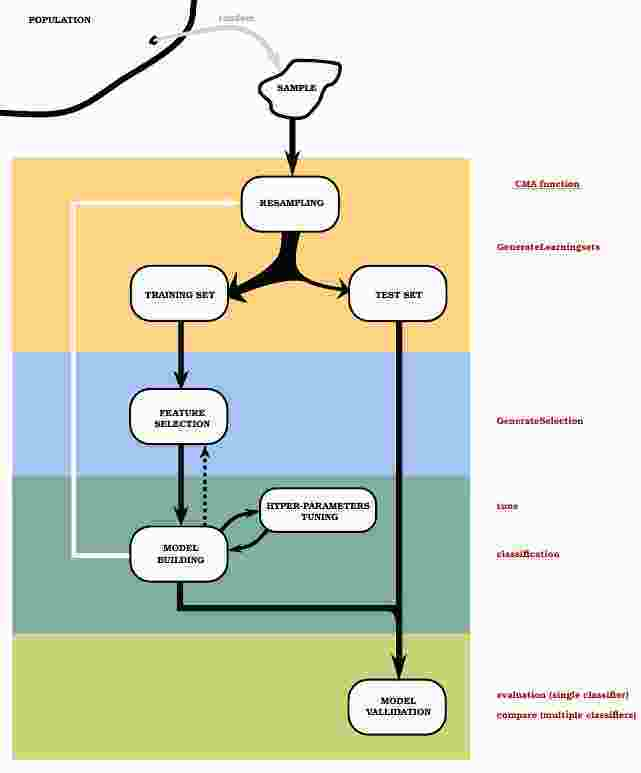
\includegraphics[width=10cm]{images/biomarkerValidationScheme}
\label{validation}
\end{figure}

\subsection{The CMA package}

There are many packages in \R to apply each of the many available
classification methods.  Some of them such as \texttt{caret}
(\ref{caretPackage}), \texttt{CMA} (\ref{cmaPackage}) or
\texttt{MLtools} (\ref{mltoolsPackage}) also support the process of
building and validating a classifier based on testing a set of
different approaches on a set of samples using an appropriate
cross-validation approach. 

Here we rely on the Bioconductor \texttt{CMA} (``Classification for MicroArrays'') package which has been
specifically designed with microarray data in mind, but can also be used with any high throughput data.

\begin{knitrout}
\definecolor{shadecolor}{rgb}{0.969, 0.969, 0.969}\color{fgcolor}\begin{kframe}
\begin{alltt}
\hlcom{# Compte: cal carregar abans el paquet e1071 perque si no es fa així pot donar error al mètode "tune" (els dos en tenen un que es diu així)}

\hlkwa{if} \hlstd{(}\hlopt{!}\hlkwd{require}\hlstd{(e1071))\{}
  \hlkwd{install.packages}\hlstd{(}\hlstr{"e1071"}\hlstd{,} \hlkwc{dep}\hlstd{=}\hlnum{TRUE}\hlstd{)}
\hlstd{\}}
\hlkwd{require}\hlstd{(e1071)}

\hlkwa{if} \hlstd{(}\hlopt{!}\hlkwd{require}\hlstd{(glmnet))\{}
  \hlkwd{install.packages}\hlstd{(}\hlstr{"glmnet"}\hlstd{,} \hlkwc{dep}\hlstd{=}\hlnum{TRUE}\hlstd{)}
\hlstd{\}}
\hlkwd{require}\hlstd{(glmnet)}

\hlkwa{if} \hlstd{(}\hlopt{!}\hlkwd{require}\hlstd{(randomForest))\{}
  \hlkwd{install.packages}\hlstd{(}\hlstr{"randomForest"}\hlstd{,} \hlkwc{dep}\hlstd{=}\hlnum{TRUE}\hlstd{)}
\hlstd{\}}
\hlkwd{require}\hlstd{(randomForest)}


\hlkwa{if} \hlstd{(}\hlopt{!}\hlstd{(}\hlkwd{require}\hlstd{(CMA)))\{}
  \hlkwd{source}\hlstd{(}\hlstr{"http://Bioconductor.org/biocLite.R"}\hlstd{)}
  \hlkwd{biocLite}\hlstd{(}\hlstr{"CMA"}\hlstd{)}
\hlstd{\}}
\hlkwd{require}\hlstd{(CMA)}
\end{alltt}
\end{kframe}
\end{knitrout}


According to its manual the aim of the package is \emph{to provide a
user-friendly environment for the evaluation of classification methods
using gene expression data}. A strong focus is on combined variable
selection, hyperparameter tuning, evaluation, visualization and
comparison of (up to now) 21 classification methods from three main
fields: Discriminant Analysis, Neural Networks and Machine Learning.

Using this package a (not-so-)simple workflow for building and validating a classifier can be built.
The main steps for this workflow are: 
\begin{enumerate}
\item Start with a high-throughput dataset (e.g. en expression matrix) and a vector of labels assigning each column of the dataset to a group.
\item 
Generate a given number of evaluation datasets using \texttt{GenerateLearningsets}.
\item 
(Optionally): Perform variable selection using \texttt{GeneSelection}.
\item 
(Optionally): Peform hyperparameter tuning using \texttt{tune}.
\item 
Perform classification using 1.-3.
\item 
Repeat steps 3--5 based on the learning sets generated in step 2 for an appropriate (wisely chosen) subset of all available methods\footnote{compBoostCMA, dldaCMA, ElasticNetCMA, fdaCMA, flexdaCMA, gbmCMA, knnCMA, ldaCMA, LassoCMA, nnetCMA, pknnCMA, plrCMA, pls_ldaCMA, pls_lrCMA, pls_rfCMA, pnnCMA, qdaCMA, rfCMA, scdaCMA, shrinkldaCMA, svmCMA}.
\item Evaluate the results from 6 using \texttt{evaluation} and/or compare the different results using the \texttt{compare} function.
\end{enumerate}

\textbf{In practice} in order to implement the workflow a series of decisions must be taken. This means that one has to decide:
\begin{itemize}
\item Which methods to use for building learning sets.
\item Which methods to use for selecting variables with best discriminating power.
\item How many variables to use when building those classifiers that cannot decide this by themselves.
\item Which classifiers to build so that the set of classifiers tested is simultaneosuly comprehensive (represents well different philosopies) and non-redundant (excludes equivalent or very similar methods).
\end{itemize}

This can be done using a nested loop that applies each gene selection
method for each sample size each learning set and each classifier.

\subsection{The data for the analysis}

Although the goal of this document is to be as general as possible it
is good to recall that not all datasets are suitable for
classification analysis, due mainly to the fact that problems in the
data can badly affect the performance of predictors obtained.

That is if the data to be used shows batch effects, too many variables
or outliers, this has to be dealt with before attempting to build
and compare the predictors.

Some typical preprocessing that may have to be dealt with are:
\begin{enumerate}
\item remove outliers, 
\item keep only groups of samples where there were individuals of both classes analyzed and
\item remove batch effects attributable to technical questions or to experimental design
\item filter the data to retain only genes with a "minimum" variability (that is remove "flat" features).
\end{enumerate}

Although a Bioconductor package CMA uses no Bioconductor structures
that is, it expects the data to be in a numerical matrix and the labels
to be in a character (or factor) vector.

Indeed for coherence with many standard \R packages CMA assumes that variables are in columns and samples in rows, that is, it works with what would be the transposed of standard expression matrices.

In order to keep this document as much general as possible the data used to illustrate the following sections are one of those contained in the CMA package, the \texttt{khan} dataset. It consists of expression values obtained from small blue round cell tumour which
comprises 65 samples from four tumour classes.

\begin{knitrout}
\definecolor{shadecolor}{rgb}{0.969, 0.969, 0.969}\color{fgcolor}\begin{kframe}
\begin{alltt}
\hlkwd{require}\hlstd{(CMA)}
\end{alltt}


{\ttfamily\noindent\itshape\color{messagecolor}{\#\# Loading required package: CMA}}

{\ttfamily\noindent\itshape\color{messagecolor}{\#\# Loading required package: Biobase}}

{\ttfamily\noindent\itshape\color{messagecolor}{\#\# Loading required package: BiocGenerics}}

{\ttfamily\noindent\itshape\color{messagecolor}{\#\# Loading required package: parallel}}

{\ttfamily\noindent\itshape\color{messagecolor}{\#\# \\\#\# Attaching package: 'BiocGenerics'}}

{\ttfamily\noindent\itshape\color{messagecolor}{\#\# The following objects are masked from 'package:parallel':\\\#\# \\\#\#\ \ \ \  clusterApply, clusterApplyLB, clusterCall, clusterEvalQ,\\\#\#\ \ \ \  clusterExport, clusterMap, parApply, parCapply, parLapply,\\\#\#\ \ \ \  parLapplyLB, parRapply, parSapply, parSapplyLB}}

{\ttfamily\noindent\itshape\color{messagecolor}{\#\# The following object is masked from 'package:stats':\\\#\# \\\#\#\ \ \ \  xtabs}}

{\ttfamily\noindent\itshape\color{messagecolor}{\#\# The following objects are masked from 'package:base':\\\#\# \\\#\#\ \ \ \  anyDuplicated, append, as.data.frame, as.vector, cbind, colnames,\\\#\#\ \ \ \  do.call, duplicated, eval, evalq, Filter, Find, get, intersect,\\\#\#\ \ \ \  is.unsorted, lapply, Map, mapply, match, mget, order, paste, pmax,\\\#\#\ \ \ \  pmax.int, pmin, pmin.int, Position, rank, rbind, Reduce, rep.int,\\\#\#\ \ \ \  rownames, sapply, setdiff, sort, table, tapply, union, unique,\\\#\#\ \ \ \  unlist}}

{\ttfamily\noindent\itshape\color{messagecolor}{\#\# Welcome to Bioconductor\\\#\# \\\#\#\ \ \ \  Vignettes contain introductory material; view with\\\#\#\ \ \ \  'browseVignettes()'. To cite Bioconductor, see\\\#\#\ \ \ \  'citation("{}Biobase"{})', and for packages 'citation("{}pkgname"{})'.}}\begin{alltt}
\hlkwd{data}\hlstd{(khan)}
\hlstd{nabX} \hlkwb{<-} \hlkwd{as.matrix}\hlstd{(khan[,}\hlopt{-}\hlnum{1}\hlstd{])}
\hlkwd{dim}\hlstd{(nabX)}
\end{alltt}
\begin{verbatim}
## [1]   63 2308
\end{verbatim}
\begin{alltt}
\hlstd{nabY} \hlkwb{<-} \hlstd{labs}\hlkwb{<-}\hlkwd{as.factor}\hlstd{(khan[,}\hlnum{1}\hlstd{])}
\hlkwd{table}\hlstd{(nabY)}
\end{alltt}
\begin{verbatim}
## nabY
##  BL EWS  NB RMS 
##   8  23  12  20
\end{verbatim}
\end{kframe}
\end{knitrout}

\section{Building and validating the predictors}

\subsection{Creating the learning datasets}

Ideally in classification problems one should have a completely independent test set where the classifier could be checked once it has been built on the train data. 

Given that it is not usually possible an alternative approach is to perform \emph{cross-validation} which consists of creating a certain number of splits of the data (that is different divisions of the original dataset into a train and test subset) which can later be used to train/test the predictor and whose results can be aggregated.

There are different schemes for splitting the samples into test and train subsets. Here we use  the "five-fold" and "Monte Carlo Cross-Validation" approaches, described in \cite{CMAvignette}.


\begin{knitrout}
\definecolor{shadecolor}{rgb}{0.969, 0.969, 0.969}\color{fgcolor}\begin{kframe}
\begin{alltt}
\hlcom{#### NOTA: AL FER EL CÀLCUL DEFINITIU CONVE AUGMENTAR EL NOMBRE D'ITERACIONS. (per exemple a 1000)}
\hlstd{numIter} \hlkwb{<-} \hlnum{3}
\hlstd{numFold} \hlkwb{<-} \hlnum{5}
\hlstd{learnSetNames} \hlkwb{<-} \hlkwd{c}\hlstd{(}\hlstr{"fiveFold"}\hlstd{,} \hlstr{"MCCV"}\hlstd{)}
\hlkwd{set.seed}\hlstd{(}\hlnum{1234567}\hlstd{)}
\end{alltt}
\end{kframe}
\end{knitrout}




\subsection{Selecting genes}

The first important step in the process of building a classifier is \emph{variable selection}. It is very important, however, not to confound variable selection with classification. Gene selection -or variable selection- is ``only'' intended to select appropriate variables, but tells nothing about classifiers. Classification relies on variables that distinguish well samples but it looks for a more complex information, that is the ability to classify new individuals into either groups.

Following the recommendations in \cite{Boulesteix:2010} it is a good idea to use several, different, variable selection methods that rely on different approaches, Here we try three  gene selection methods: \emph{T-test}, \emph{Random forest} and the \emph{Lasso} corresponding to three different approaches (...).

The code below shows how to perform gene selection on the different learning sets and how to annotate compare them.

This provides relevant information, but it is important to recall that it does not provide us with what is the goal of this document: a good classifier.

\begin{knitrout}
\definecolor{shadecolor}{rgb}{0.969, 0.969, 0.969}\color{fgcolor}\begin{kframe}
\begin{alltt}
\hlcom{# selMethodNames <- c("t.test", "rfe", "lasso") # VALID PER DOS GRUPS}
\hlcom{# selScheme <- "pairwise"                       # VALID PER DOS GRUPS}
\hlstd{selMethodNames} \hlkwb{<-} \hlkwd{c}\hlstd{(}\hlstr{"f.test"}\hlstd{,} \hlstr{"rf"}\hlstd{)}           \hlcom{# ADIENT PER MES DE 2 GRUPS}
\hlstd{schemeName} \hlkwb{<-} \hlstr{"multiclass"}                     \hlcom{# ADIENT PER MES DE 2 GRUPS}
\hlstd{numGenes2Sel} \hlkwb{<-} \hlkwd{c}\hlstd{(}\hlnum{2}\hlstd{,}\hlnum{5}\hlstd{,}\hlnum{10}\hlstd{,} \hlnum{25}\hlstd{)}
\end{alltt}
\end{kframe}
\end{knitrout}

\begin{knitrout}
\definecolor{shadecolor}{rgb}{0.969, 0.969, 0.969}\color{fgcolor}\begin{kframe}
\begin{alltt}
\hlcom{# Això no cal fer-ho perque es fa al loop principal}
\hlstd{geneSels}\hlkwb{<-} \hlkwd{list}\hlstd{()}
\hlkwa{for} \hlstd{(i} \hlkwa{in} \hlnum{1}\hlopt{:}\hlkwd{length}\hlstd{(learningSets))\{}
  \hlkwa{for} \hlstd{(j} \hlkwa{in} \hlnum{1}\hlopt{:}\hlkwd{length}\hlstd{(selMethodNames))\{}
    \hlstd{selected}  \hlkwb{<-} \hlkwd{GeneSelection}\hlstd{(nabX, nabY,} \hlkwc{learningsets} \hlstd{= learningSets[[i]],}
                               \hlkwc{method} \hlstd{= selMethodNames[j],} \hlkwc{scheme}\hlstd{=schemeName)}
    \hlstd{itemName}\hlkwb{<-} \hlkwd{paste}\hlstd{(learnSetNames[i], selMethodNames[j],} \hlkwc{sep}\hlstd{=}\hlstr{"."}\hlstd{)}
    \hlstd{geneSels[[itemName]]}\hlkwb{<-}\hlstd{selected}
  \hlstd{\}}
\hlstd{\}}
\end{alltt}
\begin{verbatim}
## GeneSelection: iteration 1 
## GeneSelection: iteration 2 
## GeneSelection: iteration 3 
## GeneSelection: iteration 4 
## GeneSelection: iteration 5 
## GeneSelection: iteration 6 
## GeneSelection: iteration 7 
## GeneSelection: iteration 8 
## GeneSelection: iteration 9 
## GeneSelection: iteration 10 
## GeneSelection: iteration 11 
## GeneSelection: iteration 12 
## GeneSelection: iteration 13 
## GeneSelection: iteration 14 
## GeneSelection: iteration 15 
## GeneSelection: iteration 1
\end{verbatim}


{\ttfamily\noindent\color{warningcolor}{\#\# Warning in library(package, lib.loc = lib.loc, character.only = TRUE, logical.return = TRUE, : there is no package called 'randomForest'}}

{\ttfamily\noindent\bfseries\color{errorcolor}{\#\# Error in selfun(X, y, learnind = learnmatrix[i, ], ...): could not find function "{}randomForest"{}}}\begin{alltt}
\hlstd{selectedGenesFileName} \hlkwb{<-} \hlkwd{paste}\hlstd{(}\hlstr{"selectedGenes"}\hlstd{,numIter,}\hlstr{"iter.Rda"}\hlstd{,} \hlkwc{sep}\hlstd{=}\hlstr{""}\hlstd{)}
\hlkwd{save}\hlstd{(geneSels,} \hlkwc{file}\hlstd{=}\hlkwd{file.path}\hlstd{(resultsDir,selectedGenesFileName))}
\end{alltt}
\end{kframe}
\end{knitrout}

\begin{knitrout}
\definecolor{shadecolor}{rgb}{0.969, 0.969, 0.969}\color{fgcolor}\begin{kframe}
\begin{alltt}
\hlcom{# Si no s'ha fet lo de dalt no tes sentit}
\hlkwa{if} \hlstd{(}\hlopt{!}\hlstd{(}\hlkwd{exists}\hlstd{(}\hlstr{"learningSets"}\hlstd{)))} \hlkwd{load}\hlstd{(}\hlkwc{file}\hlstd{=}\hlkwd{file.path}\hlstd{(resultsDir, learningSetsFileName))}
\hlkwa{if} \hlstd{(}\hlopt{!}\hlstd{(}\hlkwd{exists}\hlstd{(}\hlstr{"geneSels"}\hlstd{)))} \hlkwd{load}\hlstd{(}\hlkwc{file}\hlstd{=}\hlkwd{file.path}\hlstd{(resultsDir, selectedGenesFileName))}
\hlstd{topLists} \hlkwb{<-} \hlkwd{lapply}\hlstd{(geneSels, toplist,} \hlnum{25}\hlstd{)}
\end{alltt}
\begin{verbatim}
## top  25  genes for iteration  1 
##  
##    index importance
## 1   1389     61.486
## 2    246     61.435
## 3    545     50.657
## 4   1955     50.308
## 5    842     42.971
## 6   1954     39.999
## 7   2050     38.351
## 8   1003     37.919
## 9    107     36.631
## 10  1194     36.296
## 11  1319     35.269
## 12   129     33.405
## 13   509     33.352
## 14   187     32.890
## 15  1066     32.807
## 16  1158     32.435
## 17   255     30.925
## 18  2046     30.462
## 19   742     30.039
## 20     1     30.013
## 21  1427     29.658
## 22  1980     29.240
## 23  1207     28.783
## 24  1645     27.718
## 25  1708     27.107
\end{verbatim}
\begin{alltt}
\hlstd{res25}\hlkwb{<-} \hlkwd{as.data.frame}\hlstd{(topLists)}
\hlkwd{colnames}\hlstd{(res25)}
\end{alltt}
\begin{verbatim}
## [1] "fiveFold.f.test.index"      "fiveFold.f.test.importance"
\end{verbatim}
\begin{alltt}
\hlstd{res.ftest} \hlkwb{<-} \hlkwd{c}\hlstd{(res25[,}\hlnum{1}\hlstd{], res25[,}\hlnum{5}\hlstd{])}
\end{alltt}


{\ttfamily\noindent\bfseries\color{errorcolor}{\#\# Error in `[.data.frame`(res25, , 5): undefined columns selected}}\begin{alltt}
\hlstd{res.rf} \hlkwb{<-}  \hlkwd{c}\hlstd{(res25[,}\hlnum{3}\hlstd{], res25[,}\hlnum{7}\hlstd{])}
\end{alltt}


{\ttfamily\noindent\bfseries\color{errorcolor}{\#\# Error in `[.data.frame`(res25, , 3): undefined columns selected}}\begin{alltt}
\hlstd{res.all} \hlkwb{<-} \hlkwd{c}\hlstd{(res.ftest, res.rf)}
\end{alltt}


{\ttfamily\noindent\bfseries\color{errorcolor}{\#\# Error in eval(expr, envir, enclos): object 'res.ftest' not found}}\begin{alltt}
\hlkwd{table}\hlstd{(res.ftest)}
\end{alltt}


{\ttfamily\noindent\bfseries\color{errorcolor}{\#\# Error in eval(expr, envir, enclos): object 'res.ftest' not found}}\begin{alltt}
\hlkwd{table}\hlstd{(res.rf)}
\end{alltt}


{\ttfamily\noindent\bfseries\color{errorcolor}{\#\# Error in eval(expr, envir, enclos): object 'res.rf' not found}}\begin{alltt}
\hlkwd{table}\hlstd{(res.all)}
\end{alltt}


{\ttfamily\noindent\bfseries\color{errorcolor}{\#\# Error in eval(expr, envir, enclos): object 'res.all' not found}}\begin{alltt}
\hlstd{x}\hlkwb{<-}\hlkwd{as.data.frame}\hlstd{(}\hlkwd{sort}\hlstd{(}\hlkwd{table}\hlstd{(res.all),} \hlkwc{decreasing}\hlstd{=}\hlnum{TRUE}\hlstd{))}
\end{alltt}


{\ttfamily\noindent\bfseries\color{errorcolor}{\#\# Error in as.data.frame(sort(table(res.all), decreasing = TRUE)): error in evaluating the argument 'x' in selecting a method for function 'as.data.frame': Error in sort(table(res.all), decreasing = TRUE) : \\\#\#\ \  error in evaluating the argument 'x' in selecting a method for function 'sort': Error in eval(expr, envir, enclos) : object 'res.all' not found\\\#\# Calls: table -> standardGeneric -> eval -> eval -> eval}}\begin{alltt}
\hlcom{# require(annotate)}
\hlcom{# require("hgu133plus2.db")}
\hlcom{# gname <- function(x) unlist(mget(x, hgu133plus2GENENAME))}
\hlcom{# gsymb <- function(x) getSYMBOL(x, "hgu133plus2.db")}
\hlcom{# genIdxs <- rownames(x)}
\hlcom{# geneNames <- colnames(nabX)}
\hlcom{# myGeneNames <- geneNames[as.integer(genIdxs)]}
\hlcom{# myGeneSymbols <- gsymb(myGeneNames)}
\hlcom{# myGeneDesc <- gname(myGeneNames)}
\hlcom{# selectedTable <- cbind(Gene=myGeneSymbols, as.integer(x[,1]), Desc=myGeneDesc)}
\hlkwd{colnames}\hlstd{(x)} \hlkwb{<-} \hlstd{timesSelected}
\end{alltt}


{\ttfamily\noindent\bfseries\color{errorcolor}{\#\# Error in eval(expr, envir, enclos): object 'timesSelected' not found}}\begin{alltt}
\hlstd{selectedTable} \hlkwb{<-} \hlstd{x}
\end{alltt}


{\ttfamily\noindent\bfseries\color{errorcolor}{\#\# Error in eval(expr, envir, enclos): object 'x' not found}}\begin{alltt}
\hlstd{biomarkersFileName} \hlkwb{<-} \hlkwd{paste}\hlstd{(}\hlstr{"candidate.biomarkers"}\hlstd{, numIter,} \hlstr{"text"}\hlstd{,} \hlkwc{sep}\hlstd{=}\hlstr{"."}\hlstd{)}
\hlkwd{write.table}\hlstd{(selectedTable,} \hlkwc{file}\hlstd{=}\hlkwd{file.path}\hlstd{(resultsDir, biomarkersFileName),} \hlkwc{sep}\hlstd{=}\hlstr{"\textbackslash{}t"}\hlstd{,} \hlkwc{row.names}\hlstd{=}\hlnum{FALSE}\hlstd{)}
\end{alltt}


{\ttfamily\noindent\bfseries\color{errorcolor}{\#\# Error in is.data.frame(x): object 'selectedTable' not found}}\end{kframe}
\end{knitrout}

File candidate.biomarkers.3.text contains a table with genes selected by the different methods and the number of times they have been selected.

\subsection{Hyperparameter tuning}

Some methods require -it is recommended- that a tuning of their parameters is performed to yield their best performance.
To avoid overfitting this tuning is performed inside the cross-validation loop created to test each classifier on each set of (selected) variables and each set of randomly selected trainig samples.

\subsection{Classification}

Once all the elements are ready that is: cross-validation scheme, gene selection methods and hyperparameter tunings needed known a global cross-validation loop implementing the process can be builit. The CMA package has some functions that strongly facilitate this process as shown in the code below.


\begin{knitrout}
\definecolor{shadecolor}{rgb}{0.969, 0.969, 0.969}\color{fgcolor}\begin{kframe}
\begin{alltt}
\hlkwd{load}\hlstd{(}\hlkwc{file}\hlstd{=}\hlkwd{file.path}\hlstd{(resultsDir, learningSetsFileName))}
\hlcom{# load(file=file.path(resultsDir, selectedGenesFileName)) NO CAL: Es recalcula}

\hlstd{classifierNames} \hlkwb{<-} \hlkwd{c}\hlstd{(}\hlstr{"dldaCMA"}\hlstd{,} \hlstr{"knnCMA"}\hlstd{,} \hlstr{"rfCMA"}\hlstd{,} \hlstr{"scdaCMA"}\hlstd{,} \hlstr{"svmCMA"}\hlstd{)}
\hlstd{isTunable} \hlkwb{<-} \hlkwd{c}\hlstd{(}\hlnum{FALSE}\hlstd{,} \hlnum{TRUE}\hlstd{,} \hlnum{FALSE}\hlstd{,} \hlnum{TRUE}\hlstd{,} \hlnum{TRUE}\hlstd{)}

\hlcom{#classifierNames <- c("dldaCMA", "knnCMA")}
\hlcom{#isTunable <- c(FALSE, TRUE)}

\hlstd{classifs} \hlkwb{<-} \hlkwd{list}\hlstd{()}

\hlstd{st} \hlkwb{<-} \hlkwd{system.time}\hlstd{(}
\hlkwa{for} \hlstd{(i} \hlkwa{in} \hlnum{1}\hlopt{:}\hlkwd{length}\hlstd{(learningSets))\{}
  \hlkwa{for} \hlstd{(j} \hlkwa{in} \hlnum{1}\hlopt{:}\hlkwd{length}\hlstd{(selMethodNames))\{}
      \hlstd{selected}  \hlkwb{<-} \hlkwd{GeneSelection}\hlstd{(nabX, nabY,} \hlkwc{learningsets} \hlstd{= learningSets[[i]],}
                                 \hlkwc{method} \hlstd{= selMethodNames[j])}
      \hlkwa{for} \hlstd{(numGenes} \hlkwa{in} \hlstd{numGenes2Sel)\{} \hlcom{# Opcional : Un altre nivell d'iteració}
        \hlkwa{for} \hlstd{(k} \hlkwa{in} \hlnum{1}\hlopt{:}\hlkwd{length}\hlstd{(classifierNames))\{}
          \hlstd{myClassifier} \hlkwb{<-} \hlkwd{eval}\hlstd{(}\hlkwd{parse}\hlstd{(}\hlkwc{text}\hlstd{=classifierNames[k]))}
          \hlkwa{if}\hlstd{(isTunable[k])\{}
               \hlstd{tuneVals} \hlkwb{<-} \hlkwd{tune} \hlstd{(}\hlkwc{X}\hlstd{=nabX,} \hlkwc{y}\hlstd{=nabY,} \hlkwc{learningsets}\hlstd{= learningSets[[i]],}
                                 \hlkwc{genesel}\hlstd{=selected,} \hlkwc{nbgene}\hlstd{=numGenes,}
                                \hlkwc{classifier} \hlstd{=myClassifier,}  \hlkwc{grids}\hlstd{=}\hlkwd{list}\hlstd{())}
               \hlstd{classif} \hlkwb{<-} \hlkwd{classification}\hlstd{(}\hlkwc{X} \hlstd{= nabX,} \hlkwc{y}\hlstd{=nabY,} \hlkwc{learningsets} \hlstd{= learningSets[[i]],}
                                         \hlkwc{genesel}\hlstd{=selected,} \hlkwc{nbgene}\hlstd{=numGenes,}
                                         \hlkwc{classifier}\hlstd{=myClassifier,}
                                         \hlkwc{tuneres}\hlstd{=tuneVals)}
             \hlstd{\}}\hlkwa{else}\hlstd{\{}
               \hlstd{classif} \hlkwb{<-} \hlkwd{classification}\hlstd{(}\hlkwc{X} \hlstd{= nabX,} \hlkwc{y}\hlstd{=nabY,} \hlkwc{learningsets} \hlstd{= learningSets[[i]],}
                                         \hlkwc{genesel}\hlstd{=selected,} \hlkwc{nbgene}\hlstd{=numGenes,}
                                         \hlkwc{classifier}\hlstd{=myClassifier)}
             \hlstd{\}}
          \hlstd{itemName}\hlkwb{<-} \hlkwd{paste}\hlstd{(learnSetNames[i], selMethodNames[j], numGenes, classifierNames[k],} \hlkwc{sep}\hlstd{=}\hlstr{"."}\hlstd{)}
          \hlstd{classifs[[itemName]]}\hlkwb{<-} \hlstd{classif}
        \hlstd{\}}
      \hlstd{\}}
    \hlstd{\}}
\hlstd{\}}
\hlstd{)}
\end{alltt}


{\ttfamily\noindent\color{warningcolor}{\#\# Warning in tune(X, y = as.numeric(y) - 1, learningsets = learningsets, genesel = genesel, : Combination of feature selection and hyperparameter tuning\\\#\#\ \ \ \ \ \ \ \ \ \ \ \ \ \ \ \ is subject to pessimistic bias and will be fixed in a future\\\#\#\ \ \ \ \ \ \ \ \ \ \ \ \ \ \ \ package version.}}

{\ttfamily\noindent\color{warningcolor}{\#\# Warning: package 'class' was built under R version 3.1.3}}

{\ttfamily\noindent\color{warningcolor}{\#\# Warning in library(package, lib.loc = lib.loc, character.only = TRUE, logical.return = TRUE, : there is no package called 'randomForest'}}

{\ttfamily\noindent\bfseries\color{errorcolor}{\#\# Error in classifier(models = FALSE, X = structure(c(1.183075979, 0.545111102, : could not find function "{}randomForest"{}}}\begin{alltt}
\hlkwd{cat}\hlstd{(}\hlstr{"Time consumed: "}\hlstd{, st,} \hlstr{"\textbackslash{}n"}\hlstd{)}
\end{alltt}


{\ttfamily\noindent\bfseries\color{errorcolor}{\#\# Error in cat("{}Time consumed: "{}, st, "{}\textbackslash{}n"{}): object 'st' not found}}\begin{alltt}
\hlstd{classifsFileName} \hlkwb{<-} \hlkwd{paste}\hlstd{(}\hlstr{"classifs"}\hlstd{,numIter,}\hlstr{"iter.Rda"}\hlstd{,} \hlkwc{sep}\hlstd{=}\hlstr{""}\hlstd{)}
\hlkwd{save}\hlstd{(classifs,} \hlkwc{file}\hlstd{=}\hlkwd{file.path}\hlstd{(resultsDir,classifsFileName))}
\end{alltt}
\end{kframe}
\end{knitrout}

\subsection{Classifiers comparison}

The loop performed in the previous section builds and tests many different classifiers. In order to evaluate and compare them they can be processed using the CMA function \texttt{compare} which analyzes the performance of each classifier based on standard measures such as "misclassification probability", "sensitivity", "specificity" or the ``auc'' the area under the curve.

Classification results can be plotted or stored in a file for further exploration

\begin{knitrout}
\definecolor{shadecolor}{rgb}{0.969, 0.969, 0.969}\color{fgcolor}\begin{kframe}
\begin{alltt}
\hlstd{compMeasures} \hlkwb{<-}  \hlkwd{c}\hlstd{(}\hlstr{"misclassification"}\hlstd{,} \hlstr{"sensitivity"}\hlstd{,} \hlstr{"specificity"}\hlstd{)}
                  \hlcom{# , "average probability", "auc")}
\hlstd{s1} \hlkwb{<-} \hlkwd{c}\hlstd{(}\hlkwd{rep}\hlstd{(}\hlstr{"fiveF"}\hlstd{,} \hlnum{60}\hlstd{),} \hlkwd{rep}\hlstd{(}\hlstr{"mccv"}\hlstd{,} \hlnum{60}\hlstd{))}
\hlstd{s2}\hlkwb{<-} \hlkwd{c}\hlstd{(}\hlkwd{rep}\hlstd{(}\hlstr{"tttest"}\hlstd{,}\hlnum{20}\hlstd{),} \hlkwd{rep} \hlstd{(}\hlstr{"rfe"}\hlstd{,}\hlnum{20}\hlstd{) ,}\hlkwd{rep}\hlstd{(}\hlstr{"lasso"}\hlstd{,}\hlnum{20}\hlstd{),}
       \hlkwd{rep}\hlstd{(}\hlstr{"tttest"}\hlstd{,}\hlnum{20}\hlstd{),} \hlkwd{rep}\hlstd{(}\hlstr{"rfe"}\hlstd{,}\hlnum{20}\hlstd{),} \hlkwd{rep}\hlstd{(}\hlstr{"lasso"}\hlstd{,}\hlnum{20}\hlstd{))}
\hlstd{s3} \hlkwb{<-} \hlkwd{rep}\hlstd{(}\hlkwd{c}\hlstd{(}\hlkwd{rep}\hlstd{(}\hlnum{2}\hlstd{,}\hlnum{5}\hlstd{),} \hlkwd{rep}\hlstd{(}\hlnum{5}\hlstd{,}\hlnum{5}\hlstd{),}\hlkwd{rep}\hlstd{(}\hlnum{10}\hlstd{,}\hlnum{5}\hlstd{),} \hlkwd{rep}\hlstd{(}\hlnum{25}\hlstd{,}\hlnum{5}\hlstd{)),}\hlnum{6}\hlstd{)}
\hlstd{s4} \hlkwb{<-} \hlkwd{rep}\hlstd{(classifierNames,} \hlnum{24}\hlstd{)}
\hlstd{s} \hlkwb{<-} \hlkwd{paste}\hlstd{(s1,s2,s3,s4,} \hlkwc{sep}\hlstd{=}\hlstr{"."}\hlstd{)}

\hlstd{compClassifs} \hlkwb{<-} \hlkwd{compare}\hlstd{(classifs,}  \hlkwc{measure} \hlstd{= compMeasures)}
\end{alltt}


{\ttfamily\noindent\bfseries\color{errorcolor}{\#\# Error in evaluation(clresultlist[[j]], measure = measure[i]): 'sensitivity', 'specificity' or 'auc' are only computed for binary classification}}\begin{alltt}
\hlstd{resultsClassif} \hlkwb{<-} \hlkwd{data.frame}\hlstd{(}\hlkwc{CrossVal}\hlstd{=s1,} \hlkwc{VarSel}\hlstd{=s2,} \hlkwc{numGenes}\hlstd{=s3,} \hlkwc{Classif}\hlstd{=s4,compClassifs)}
\end{alltt}


{\ttfamily\noindent\bfseries\color{errorcolor}{\#\# Error in data.frame(CrossVal = s1, VarSel = s2, numGenes = s3, Classif = s4, : object 'compClassifs' not found}}\begin{alltt}
\hlkwd{write.csv2}\hlstd{(resultsClassif,} \hlkwc{file}\hlstd{=}\hlkwd{file.path}\hlstd{(resultsDir,} \hlkwd{paste}\hlstd{(}\hlstr{"resultsClassif"}\hlstd{, numIter,} \hlstr{"csv"}\hlstd{,} \hlkwc{sep}\hlstd{=}\hlstr{"."}\hlstd{)))}
\end{alltt}


{\ttfamily\noindent\bfseries\color{errorcolor}{\#\# Error in is.data.frame(x): object 'resultsClassif' not found}}\end{kframe}
\end{knitrout}

\bibliography{reviewMicroarrays} 

\end{document}
